\begin{frame}[plain]
    \begin{center}
        \vspace{48pt}
        {\huge\bf センサーについて知ろう}
    \end{center}
\end{frame}

\begin{frame}[fragile]
    \frametitle{センサーとは}
    \begin{center}
        \begin{description}
            \item 身の回りの世界の情報を調べ、コンピュータに伝える
        \end{description}
        \vspace{12pt}
        \includesvg[width=0.8\linewidth]{images/chap05/car_sensors.svg}
    \end{center}
\end{frame}

\begin{frame}[fragile]
    \frametitle{アナログ信号とデジタル信号}
    \begin{columns}
        \begin{column}{0.48\textwidth}
            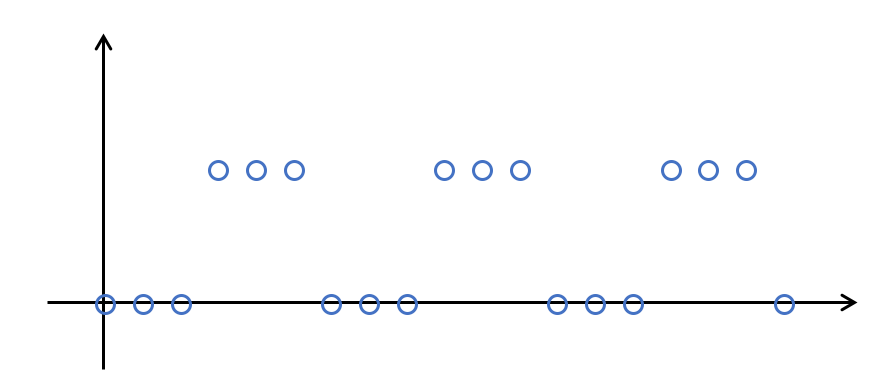
\includegraphics[width=\textwidth]{images/chap05/text05-img002.png} 
            {デジタル信号の例}
            \vspace{2pt}
            \begin{itemize}
                \item 授業で使われるデジタル信号は0と1で表すことができる
                \item 二通りのことを表すときに使う
                \item ボタンやスイッチ
            \end{itemize}
        \end{column}
        \begin{column}{0.48\textwidth}
            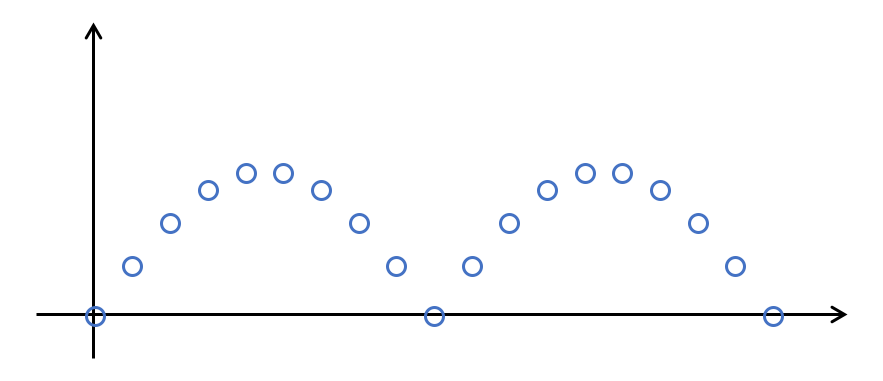
\includegraphics[width=\textwidth]{images/chap05/text05-img003.png} 
            {アナログ信号の例}
            \vspace{2pt}
            \begin{itemize}
                \item 授業で使われるアナログ信号は0〜1023の数字で表すことができる
                \item 数を表すときに使う
                \item 明るさや距離
            \end{itemize}
        \end{column}
    \end{columns}
\end{frame}

\begin{frame}[fragile]
    \frametitle{問題を解いてみよう}
    \begin{itemize}
        \item 教科書3ページ 問題5-1
        \begin{itemize}
            \item 3問
        \end{itemize}
    \end{itemize}
\end{frame}
